\chapter{関連研究}\label{chap:related}

\section{HumanComputation /
Crowdsourcing}\label{humancomputation-crowdsourcing}

コンピュータの計算能力だけでは解決できない問題を、人間の処理能力を計算資源として利用することによって解決する手法は、
ヒューマンコンピュテーション\cite{humancomputation}と呼ばれ、様々な研究が行なわれている。

reCAPTCHA\cite{recaptcha}は、

Duolingo\cite{duolingo}は、

Vizwiz\cite{vizwiz}は、

Soylent\cite{soylent}は、

\section{CrowdSourcing}\label{crowdsourcing}

インターネットを介して不特定多数の人間に仕事を依頼する仕組みはクラウドソーシングと呼ばれ、近年注目を浴びている。
クラウドソーシングとは、業務の一部を外部に委託することを示すアウトソーシングという言葉を改変した造語である\cite{riseofcrowdsourcing}。
インターネットを介した不特定多数の人間たち(crowd)に仕事をアウトソースすることから、crowdsourcingと呼ぶ。
非常に安価で、かつ、必要な人員をすぐに確保して仕事依頼が可能なことから、多くの利用例が生まれている。
近年では、Amazon Mechanical
Turk\cite{amt}(以降MTurk)等のクラウドソーシングプラットフォームが登場してきたことによって
多くの利用例が生まれている。
その中でも、本研究と類似している研究について、述べる。

\subsection{Turkit}\label{subsubsec:turkit}

Littleらは、このMTurkをプログラムから簡単に利用するためのツールキットであるTurkit\cite{turkit}を提案している。
Turkitでは、通常のプログラミング記法と同じような記法でタスクをクラウドソーシングすることができる\ref{fig:turkit}。
また、クラウドソーシングによる処理結果の保存をしておくことで、その後の処理でプログラム実行に失敗しても
再度クラウドソーシングに処理依頼をするのではなく、保存済みの結果を元にプログラムを再度実行できるような仕組み
であるthe crash-and-return プログラミングモデルを提唱している。
可能な限り従来のプログラミング記法を崩さずに人力処理を組み込むことを目的としており、本研究と類似している。
本研究は、クラウドソーシング処理を前提としておらず、特定の個人に対する指示を実現するものである。
Turkitでは特定個人に対する処理依頼を記述することはできない。
また、MTurkに依存しているため、クライアントサイドなどを自由に記述することはできない。

\begin{figure}[htbp]
  \begin{center}
  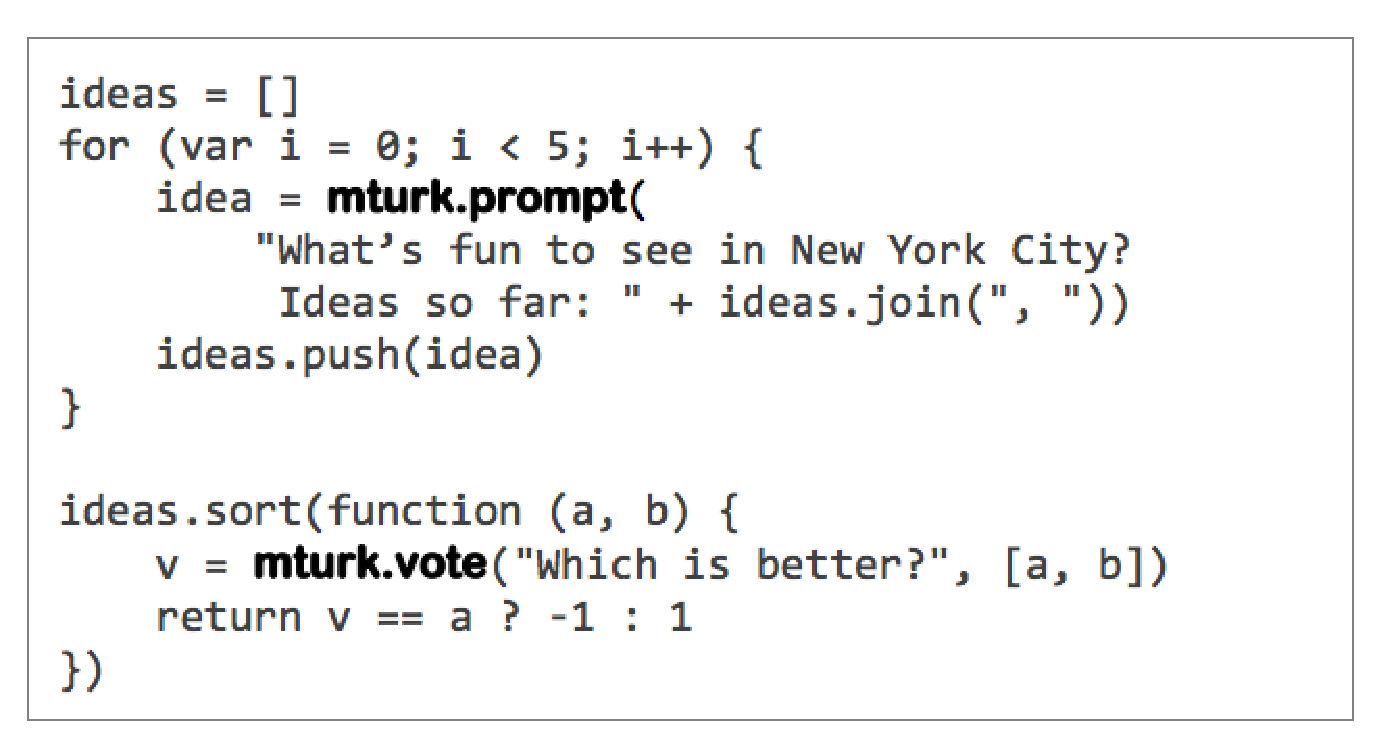
\includegraphics[width=.6\linewidth]{images/turkit.eps}
  \end{center}
  \caption{Turkit}
  \label{fig:turkit}
\end{figure}

\subsection{Automan}\label{automan}

Barowyらは、Automanというプログラミング言語Scala上で動作するDomain
Specific Languageを提案した\cite{automan}。
可能な限り通常のプログラミング記法を崩さずにクラウドソーシングを活用した人力処理を組み込むことを目的としており、
クラウドソーシングによる計算とコンピュータによる計算を統合したCrowdProgrammingを提案している。
また、回答の品質管理機能やタスクのスケジューリング、予算の配分等に関する機能を持つ。
本研究における目的は人間と計算機への指示を融合させたプログラミングを実現させることとなっており、類似している。
クラウドソーシング利用を前提としている点や、クライアントアプリケーションを自由に作ることができない点などにおいて
本研究との違いである。

\begin{figure}[htbp]
  \begin{center}
  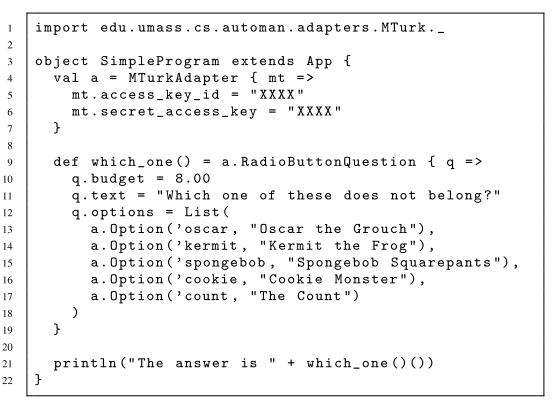
\includegraphics[width=.6\linewidth,bb=0 0 552 404]{images/automan.png}
  \end{center}
  \caption{Automan}
  \label{fig:automan}
\end{figure}

Franklinらは、CrowdDBというSQLを拡張した。

不明瞭であったり、不完全なデータの処理や、抽象的な比較 \cite{crowddb}

\cite{cylog} \cite{crowdforge} \cite{community-based-crowdsourcing}
\cite{realtime-captioning}

クラウドソーシング分野の研究では、インターネットを介して不特定多数の人を計算資源として利用することによって、
コンピュータのみでは実現できなかったような処理や、より大規模な人力処理を実現させている。
本研究では、不特定多数の人ではなく、特定可能な人を対象としたものである。

\section{Social Computing}\label{social-computing}

コンピュータ・ネットワーク上における群衆の様々な行動や叡智をフィードバックデータとして
システムに組み込み活用していくことはソーシャルコンピューティングと呼ばれている。
例えば、群衆による叡智が集められた情報をまとめるためのプラットフォームとしてはWiki\cite{wiki}が存在する。
また、人々が作るwebページのリンク関係から重要度を算出するアルゴリズムとしては、\cite{pagerank}が存在する。
また、群衆の嗜好情報等を蓄積し、個人間の嗜好等の類似度から情報の推薦等を行う手法は協調フィルタリングと呼ばれる\cite{collaborative-filtering}。

次に、特に本研究と関連するソーシャルコンピューティングの事例を紹介する。

\cite{dog}, \cite{jabberwocky}, \cite{social-machines},
\cite{personal-api},

\section{Human as Sensor}\label{human-as-sensor}

人間をセンサー代わりにしたり、人間が持つスマートフォン等のデバイスのセンサーを利用する手法はHuman
as Sensorと呼ばれる。

\cite{prism} \cite{moboq} Raらは、medusa\cite{Ra-medusa}という
Huらは、\cite{Hu:mobilecrowdsensing}

\section{Human as Actuator}\label{human-as-actuator}

アクチュエータ技術は進歩しているが、未だに人間のような汎用的に実世界に干渉できる装置はない。
そこで、人間をアクチュエータの代替として利用し動かす、つまり、人間とロボットの協調によって問題を解決しようという研究がある。

\subsection{Hapticturk}\label{hapticturk}

Hapticturk\cite{hapticturk}は、人間をモーションプラットフォームのモーターやメカニカル機構の代わりに使うことによって、
モーションプラットフォームの動きを再現するというものだ。
人間への動きの指示はスマートフォンなどを経由して行なわれる。
人間をアクチュエータの代わりに利用するといった点において、本研究と類似している。
本研究では、その用途をアクチュエータに限ったものではない。
また、プログラム上で汎用的に利用可能である。
Hapticturkでは、ゲームにその用途を限定している。

\begin{figure}[htbp]
  \begin{center}
  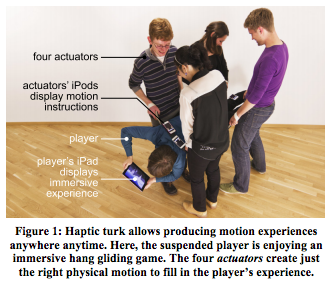
\includegraphics[width=.6\linewidth,bb=0 0 332 281]{images/hapticturk.png}
  \end{center}
  \caption{Hapticturk}
  \label{fig:hapticturk}
\end{figure}

\subsection{Sharedo}\label{sharedo}

加藤らは、ユーザとロボット間のタスクの分業

\cite{sharedo}

\subsection{グラフィカルデータフローによる調理レシピプログラミング言語の提案}\label{ux30b0ux30e9ux30d5ux30a3ux30abux30ebux30c7ux30fcux30bfux30d5ux30edux30fcux306bux3088ux308bux8abfux7406ux30ecux30b7ux30d4ux30d7ux30edux30b0ux30e9ux30dfux30f3ux30b0ux8a00ux8a9eux306eux63d0ux6848}

吉川らは調理レシピを記述するためのデータフロープログラミング言語を提案している\cite{recipe-programming}。
料理レシピをグラフィカルなデータフローで記述する。
料理レシピプログラムは、コンピュータではなく人間が実行するためのも
のだ。
本研究のように、人間がプログラムからの指示を実行することを前提としたものとなっている。

\subsection{Cooky}\label{cooky}

Sugiuraらは、人間とロボットが協調して調理をするシステムCooky\cite{cooky}を提案している。
料理支援ロボットと人とロボットが共有可能な調理器具やキッチン、調理手順を記述するシステムから成り立っている。
調理手順記述システムでは、人間とロボット双方の処理を分けて記述することができる。
人間とロボットが協調して作業を実行していくモデルは、本研究が目的とするモデルと類似する。
また、人間の作業タイミング時に、人間に作業内容を提示するなど、類似する点は多い。

\begin{figure}[htbp]
  \begin{center}
  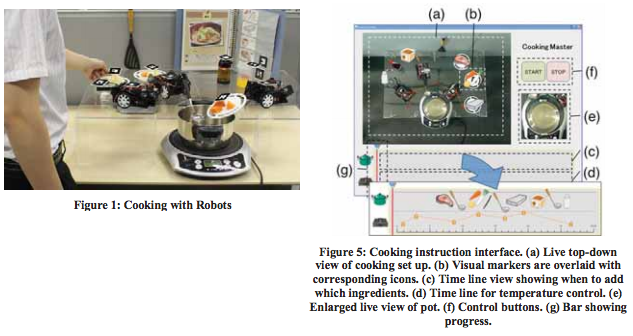
\includegraphics[width=.6\linewidth,bb=0 0 633 336]{images/cooky.png}
  \end{center}
  \caption{Cooky}
  \label{fig:cooky}
\end{figure}

\section{ワークフロー系}\label{ux30efux30fcux30afux30d5ux30edux30fcux7cfb}

仕事などにおけるプロセスを文書などによってパターンとして規定し、検証や再利用しやすくするためのものとして
ワークフローというものがある。
このワークフローを構築するための仕組みが複数存在する。

YAWL\cite{yawl}は、ワークフローやビジネス・プロセスを記述するためのワークフロー記述言語だ。
類似のものとしては、XPDL(XML Process Definition
Language)\cite{xpdl}が存在する。
これらのワークフロー記述言語を実行するワークフローエンジンと呼ばれるソフトウェアも多く存在する。
ワークフロー記述言語は、ワークフローを記述するものである。
プログラムによる処理を記述することはできない。

また、X-point\footnote{https://www.atled.jp/xpoint/}や
questetra\footnote{http://www.questetra.com/ja/}といった
ワークフロー記述・実行のためのWebサービスも存在する。
